\documentclass[12pt,letterpaper]{article}
\usepackage{graphicx,textcomp}
\usepackage{natbib}
\usepackage{setspace}
\usepackage{fullpage}
\usepackage{color}
\usepackage[reqno]{amsmath}
\usepackage{amsthm}
\usepackage{fancyvrb}
\usepackage{amssymb,enumerate}
\usepackage[all]{xy}
\usepackage{endnotes}
\usepackage{lscape}
\newtheorem{com}{Comment}
\usepackage{float}
\usepackage{hyperref}
\newtheorem{lem} {Lemma}
\newtheorem{prop}{Proposition}
\newtheorem{thm}{Theorem}
\newtheorem{defn}{Definition}
\newtheorem{cor}{Corollary}
\newtheorem{obs}{Observation}
\usepackage[compact]{titlesec}
\usepackage{dcolumn}
\usepackage{tikz}
\usetikzlibrary{arrows}
\usepackage{multirow}
\usepackage{xcolor}
\newcolumntype{.}{D{.}{.}{-1}}
\newcolumntype{d}[1]{D{.}{.}{#1}}
\definecolor{light-gray}{gray}{0.65}
\usepackage{url}
\usepackage{listings}
\usepackage{color}

\definecolor{codegreen}{rgb}{0,0.6,0}
\definecolor{codegray}{rgb}{0.5,0.5,0.5}
\definecolor{codepurple}{rgb}{0.58,0,0.82}
\definecolor{backcolour}{rgb}{0.95,0.95,0.92}

\lstdefinestyle{mystyle}{
	backgroundcolor=\color{backcolour},   
	commentstyle=\color{codegreen},
	keywordstyle=\color{magenta},
	numberstyle=\tiny\color{codegray},
	stringstyle=\color{codepurple},
	basicstyle=\footnotesize,
	breakatwhitespace=false,         
	breaklines=true,                 
	captionpos=b,                    
	keepspaces=true,                 
	numbers=left,                    
	numbersep=5pt,                  
	showspaces=false,                
	showstringspaces=false,
	showtabs=false,                  
	tabsize=2
}
\lstset{style=mystyle}
\newcommand{\Sref}[1]{Section~\ref{#1}}
\newtheorem{hyp}{Hypothesis}

\title{PS03 - My Answers (Quants 1)}
\date{13.11. 2025}
\author{Sarah Magdihs}


\begin{document}
	\maketitle
	
\section*{Question 1}
\vspace{.25cm}
\noindent We are interested in knowing how the difference in campaign spending between incumbent and challenger affects the incumbent's vote share. 
	\begin{enumerate}
		\item Run a regression where the outcome variable is \texttt{voteshare} and the explanatory variable is \texttt{difflog}.

		
		\noindent{\texttt{Answer:}} 
			\noindent {So, let's run the first regression. }
			\noindent{\texttt{R Code:}} 
		 	\lstinputlisting[language=R, firstline=58, lastline=59]{PS03_answersSM.R}  
		\noindent {This gives us the following output:}
		\begin{table}[H] \centering 
			\caption{} 
			\label{} 
			\begin{tabular}{@{\extracolsep{5pt}}lc} 
				\\[-1.8ex]\hline 
				\hline \\[-1.8ex] 
				& \multicolumn{1}{c}{\textit{Dependent variable:}} \\ 
				\cline{2-2} 
				\\[-1.8ex] & voteshare \\ 
				\hline \\[-1.8ex] 
				difflog & 0.042$^{***}$ \\ 
				& (0.001) \\ 
				& \\ 
				Constant & 0.579$^{***}$ \\ 
				& (0.002) \\ 
				& \\ 
				\hline \\[-1.8ex] 
				Observations & 3,193 \\ 
				R$^{2}$ & 0.367 \\ 
				Adjusted R$^{2}$ & 0.367 \\ 
				Residual Std. Error & 0.079 (df = 3191) \\ 
				F Statistic & 1,852.791$^{***}$ (df = 1; 3191) \\ 
				\hline 
				\hline \\[-1.8ex] 
				\textit{Note:}  & \multicolumn{1}{r}{$^{*}$p$<$0.1; $^{**}$p$<$0.05; $^{***}$p$<$0.01} \\ 
			\end{tabular} 
		\end{table} 
		
		\noindent {As we can see here, the intercept is 0.579 and the slope is 0.042. Both are statistically significant at the 0.01 level. Thus, if the spending difference is zero, the expected vote share for the incumbent is 57.9 \%. Moreover, the regression shows that for every one-unit increase in the difference in campaign spending, the incumbent’s vote share increases, on average, by 4.2 percentage points. Hence, we can infer that incumbents that outspend their challengers tend to receive more votes. Or put differently, a greater difference in campaign spending between incumbent and challenger is positively associated with a higher vote share for the incumbent. }
		
		\vspace{.25cm}
		
		
		\item Make a scatterplot of the two variables and add the regression line. 	
		
			\noindent{\texttt{Answer:}} 
		\noindent {Let's save the scatterplot next. }
		\noindent{\texttt{R Code:}} 
		\lstinputlisting[language=R, firstline=63, lastline=80]{PS03_answersSM.R} 
		\noindent {Here is the first plot: 
		
		As you can see below, the plot visually represent the output of the regression that was run in Task 1. I initially created the plot using a base R function, but eventually decided that they would look better using \textit{ggplot2}. }
			
				\vspace{.25cm}
		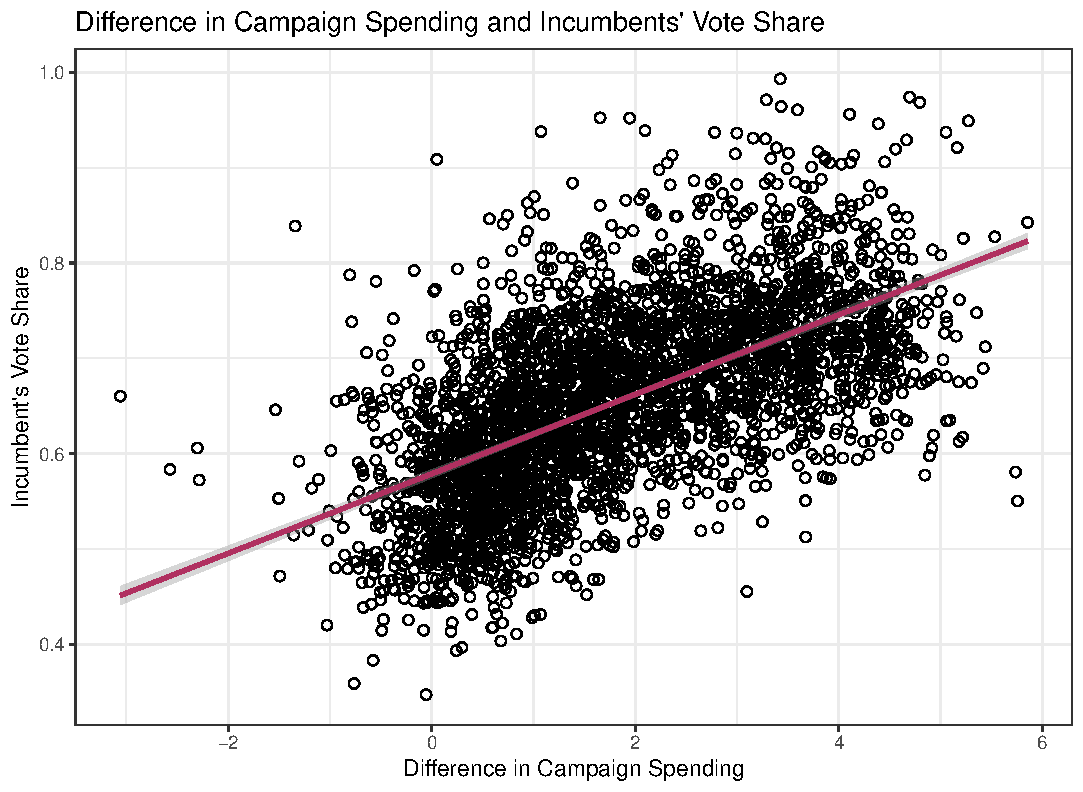
\includegraphics[width=0.8\textwidth]{plot1.pdf} 
			\vspace{.25cm}
			
		\item Save the residuals of the model in a separate object.	
		
			\noindent{\texttt{Answer:}} 
		\noindent {Let's do that as well. }
		\noindent{\texttt{R Code:}} 
				\lstinputlisting[language=R, firstline=81, lastline=82]{PS03_answersSM.R} 
		
	\item Write the prediction equation.
		
			\noindent{\texttt{Answer:}} 
		\noindent The prediction equation is: 	\[
		\widehat{\text{voteshare}} = 0.579 + 0.042 \times \text{difflog}.
		\]
	
	\end{enumerate}
	
\newpage

\section*{Question 2}
\noindent We are interested in knowing how the difference between incumbent and challenger's spending and the vote share of the presidential candidate of the incumbent's party are related.	
	\begin{enumerate}
		\item Run a regression where the outcome variable is \texttt{presvote} and the explanatory variable is \texttt{difflog}.	
		
			\noindent{\texttt{Answer:}} 
		\noindent {So, let's run the first regression. }
		\noindent{\texttt{R Code:}} 
		\lstinputlisting[language=R, firstline=96, lastline=97]{PS03_answersSM.R}  
		\noindent {This gives us the following output:}
		
		\begin{table}[H] \centering 
			\caption{} 
			\label{} 
			\begin{tabular}{@{\extracolsep{5pt}}lc} 
				\\[-1.8ex]\hline 
				\hline \\[-1.8ex] 
				& \multicolumn{1}{c}{\textit{Dependent variable:}} \\ 
				\cline{2-2} 
				\\[-1.8ex] & presvote \\ 
				\hline \\[-1.8ex] 
				difflog & 0.024$^{***}$ \\ 
				& (0.001) \\ 
				& \\ 
				Constant & 0.508$^{***}$ \\ 
				& (0.003) \\ 
				& \\ 
				\hline \\[-1.8ex] 
				Observations & 3,193 \\ 
				R$^{2}$ & 0.088 \\ 
				Adjusted R$^{2}$ & 0.088 \\ 
				Residual Std. Error & 0.110 (df = 3191) \\ 
				F Statistic & 307.715$^{***}$ (df = 1; 3191) \\ 
				\hline 
				\hline \\[-1.8ex] 
				\textit{Note:}  & \multicolumn{1}{r}{$^{*}$p$<$0.1; $^{**}$p$<$0.05; $^{***}$p$<$0.01} \\ 
			\end{tabular} 
		\end{table} 
		
		\noindent {As we can see here, the intercept is 0.508 and the slope is 0.024. Both are statistically significant at the 0.01 level. Thus, if the spending difference is zero, the expected vote share for the presidential candidate of the incumbent’s party is 50.8\%. Moreover, the regression shows that for every one-unit increase in the difference in campaign spending, the presidential candidate’s vote share increases, on average, by 2.4 percentage points. Hence, we can infer that the difference in campaign spending between incumbent and challenger is positively associated with the vote share of the presidential candidate of the incumbent’s party. It should be noted however, that this explanatory variable only explains about 8.8 \% of variation, as indicated by the R-squared value.}
		
		\item Make a scatterplot of the two variables and add the regression line. 
		
			\noindent{\texttt{Answer:}} 
		\noindent {Let's save the scatterplot next. }
		\noindent{\texttt{R Code:}} 
		\lstinputlisting[language=R, firstline=100, lastline=106]{PS03_answersSM.R} 
		\noindent {Here is the second plot: 
			
			As you can see below, the plot visually represent the output of the regression that was run in Task 1.}
		
		\vspace{.25cm}
		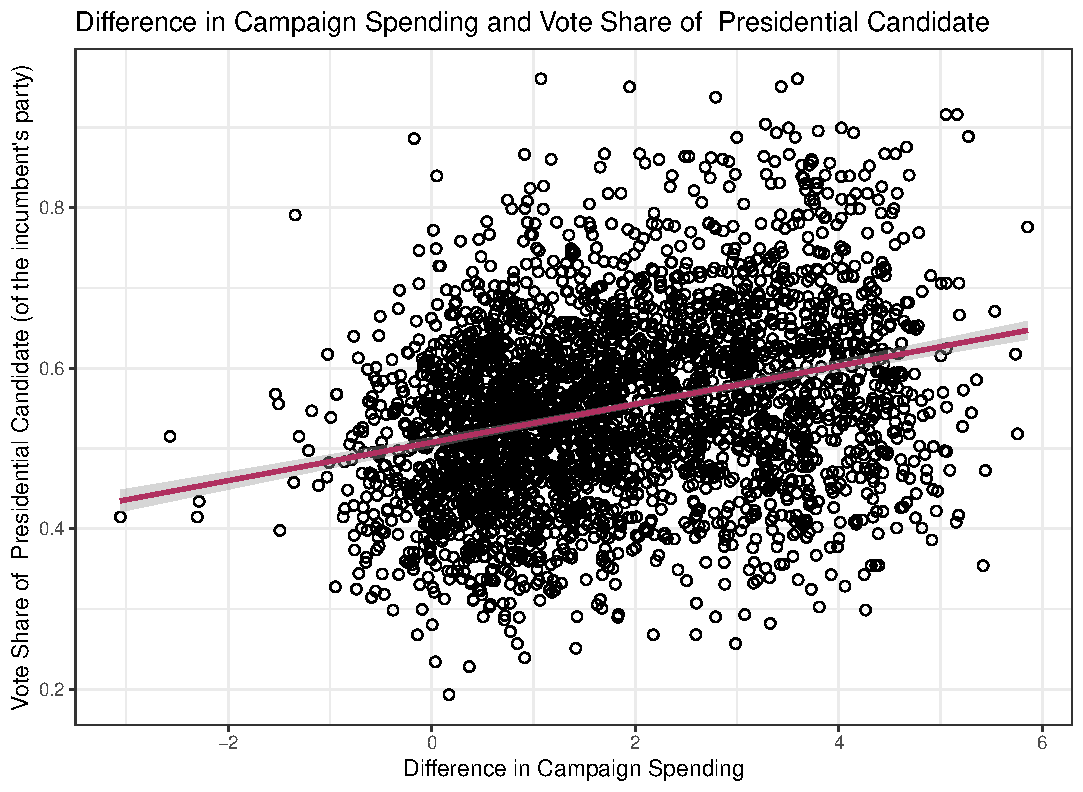
\includegraphics[width=0.8\textwidth]{plot2.pdf} 
		\vspace{.25cm}
		
			\item Save the residuals of the model in a separate object.	
		
		\noindent{\texttt{Answer:}} 
		\noindent {Let's do that as well. }
		\noindent{\texttt{R Code:}} 
		\lstinputlisting[language=R, firstline=107, lastline=108]{PS03_answersSM.R} 
		
		\item Write the prediction equation.
		
		
			\noindent{\texttt{Answer:}} 
		\noindent The prediction equation is:	\[
		\widehat{presvote} = 0.508 + 0.024 \times difflog
		\]
	\end{enumerate}
	

\section*{Question 3}

\noindent We are interested in knowing how the vote share of the presidential candidate of the incumbent's party is associated with the incumbent's electoral success.
	\vspace{.25cm}
	\begin{enumerate}
		\item Run a regression where the outcome variable is \texttt{voteshare} and the explanatory variable is \texttt{presvote}.
		
		\noindent{\texttt{Answer:}} 
		\noindent {So, let's run the first regression. }
		\noindent{\texttt{R Code:}} 
		\lstinputlisting[language=R, firstline=120, lastline=121]{PS03_answersSM.R}  
		\noindent {This gives us the following output:}
		
		\begin{table}[H] \centering 
			\caption{} 
			\label{} 
			\begin{tabular}{@{\extracolsep{5pt}}lc} 
				\\[-1.8ex]\hline 
				\hline \\[-1.8ex] 
				& \multicolumn{1}{c}{\textit{Dependent variable:}} \\ 
				\cline{2-2} 
				\\[-1.8ex] & voteshare \\ 
				\hline \\[-1.8ex] 
				presvote & 0.388$^{***}$ \\ 
				& (0.013) \\ 
				& \\ 
				Constant & 0.441$^{***}$ \\ 
				& (0.008) \\ 
				& \\ 
				\hline \\[-1.8ex] 
				Observations & 3,193 \\ 
				R$^{2}$ & 0.206 \\ 
				Adjusted R$^{2}$ & 0.206 \\ 
				Residual Std. Error & 0.088 (df = 3191) \\ 
				F Statistic & 826.950$^{***}$ (df = 1; 3191) \\ 
				\hline 
				\hline \\[-1.8ex] 
				\textit{Note:}  & \multicolumn{1}{r}{$^{*}$p$<$0.1; $^{**}$p$<$0.05; $^{***}$p$<$0.01} \\ 
			\end{tabular} 
		\end{table} 
		
			\noindent {As we can see here, the intercept is 0.441 and the slope is 0.388. Both are statistically significant at the 0.01 level. The R-squared value is 0.206, indicating that about 20.6\% of the variation in the incumbent’s vote share is explained by this model. In essence, the vote share of the presidential candidate of the incumbent’s party and the incumbent’s electoral success are positively associated with one another. Or put differently: we can infer from this regression that incumbents tend to perform better (on average) when the presidential candidate from their party receives a higher share of the vote. Note: I was - at first - a bit hesitant on how to correctly interpret the actual slope in this model, but I believe the correct interpretation (in context) is: a 0.1 increase in \texttt{presvote} (10 percentage points) is associated, on average, with a 0.0388 increase (3.88 percentage points) in the incumbent's \texttt{voteshare}.}
		
		
		\item Make a scatterplot of the two variables and add the regression line. 
			
						\noindent{\texttt{Answer:}} 
			\noindent {Let's save the scatterplot next. }
			\noindent{\texttt{R Code:}} 
			\lstinputlisting[language=R, firstline=124, lastline=133]{PS03_answersSM.R} 
			\noindent {Here is the third plot: 
				
				As you can see below, the plot visually represent the output of the regression that was run in Task 1. }
			
			\vspace{.25cm}
			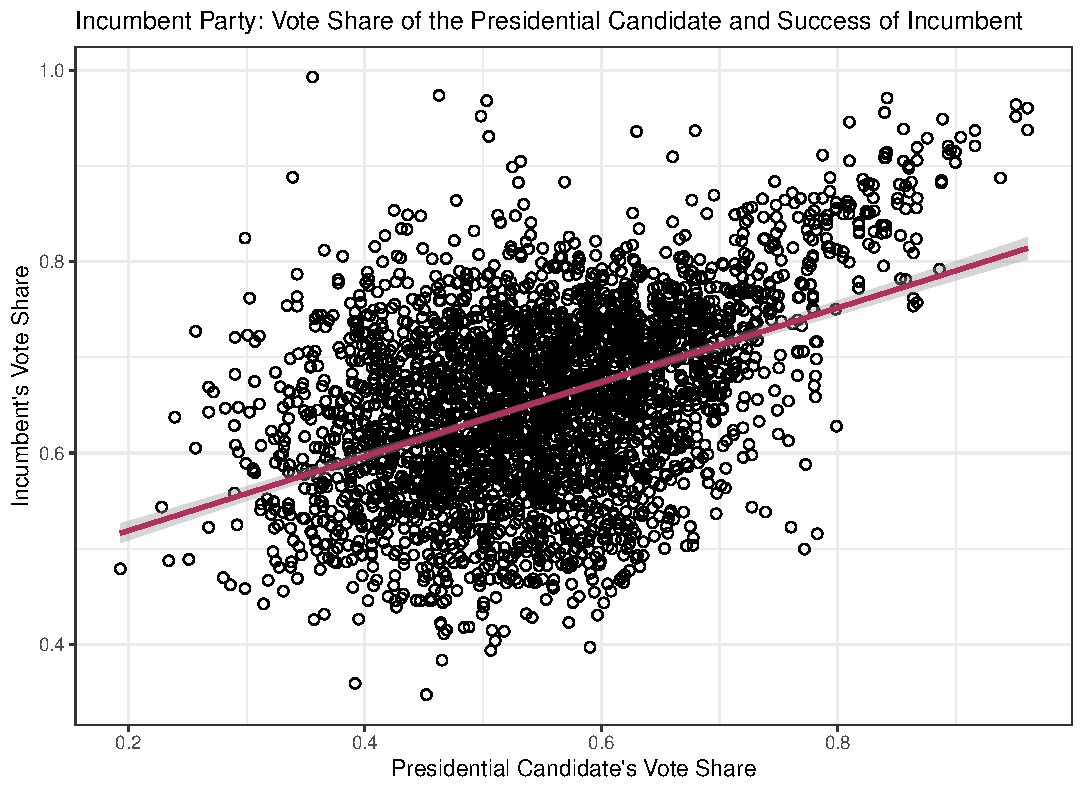
\includegraphics[width=0.8\textwidth]{plot3.pdf} 
			\vspace{.25cm}
			
			
		\item Write the prediction equation.
		
			\noindent{\texttt{Answer:}} 
		\noindent The prediction equation is: \[
		\widehat{voteshare} = 0.441 + 0.388 \times presvote
		\]
		
	\end{enumerate}

\newpage	
\section*{Question 4}
\noindent The residuals from part (a) tell us how much of the variation in \texttt{voteshare} is $not$ explained by the difference in spending between incumbent and challenger. The residuals in part (b) tell us how much of the variation in \texttt{presvote} is $not$ explained by the difference in spending between incumbent and challenger in the district.
	\begin{enumerate}
		\item Run a regression where the outcome variable is the residuals from Question 1 and the explanatory variable is the residuals from Question 2.	
		
			\noindent{\texttt{Answer:}} 
		\noindent {So, let's run the first regression. }
		\noindent{\texttt{R Code:}} 
		\lstinputlisting[language=R, firstline=144, lastline=149]{PS03_answersSM.R}  
		\noindent {This gives us the following output:}
		
		\begin{table}[H] \centering 
			\caption{} 
			\label{} 
			\begin{tabular}{@{\extracolsep{5pt}}lc} 
				\\[-1.8ex]\hline 
				\hline \\[-1.8ex] 
				& \multicolumn{1}{c}{\textit{Dependent variable:}} \\ 
				\cline{2-2} 
				\\[-1.8ex] & residuals\_1 \\ 
				\hline \\[-1.8ex] 
				residuals\_2 & 0.257$^{***}$ \\ 
				& (0.012) \\ 
				& \\ 
				Constant & $-$0.000 \\ 
				& (0.001) \\ 
				& \\ 
				\hline \\[-1.8ex] 
				Observations & 3,193 \\ 
				R$^{2}$ & 0.130 \\ 
				Adjusted R$^{2}$ & 0.130 \\ 
				Residual Std. Error & 0.073 (df = 3191) \\ 
				F Statistic & 476.975$^{***}$ (df = 1; 3191) \\ 
				\hline 
				\hline \\[-1.8ex] 
				\textit{Note:}  & \multicolumn{1}{r}{$^{*}$p$<$0.1; $^{**}$p$<$0.05; $^{***}$p$<$0.01} \\ 
			\end{tabular} 
		\end{table} 
		
			\noindent {As we can see here, the intercept is 0 and the slope is 0.257. The slope is significant at the 0.01 level. Basically, since the residuals tell us what is NOT explain in the first and second regression (which both have difflog as the explanatory variable), this regression shows the association between the residual variation of the incumbent's vote share and the presidential candidate’s vote share. The coefficient for \textit{residuals2} (the slope) is positive, which indicates that after accounting for the effects of differences in campaign spending, there is an association between \textit{presvote} and \textit{voteshare}. The R-Squared value indicates in this case that 13\% of the remaining variation in the incumbent's vote share (after accounting for difflog) is explained by the remaining variation in the presidential candidate’s vote share.}
			
			
			
		
		\item Make a scatterplot of the two residuals and add the regression line. 
		noindent{\texttt{Answer:}} 
		\noindent {Let's save the scatterplot next. }
		\noindent{\texttt{R Code:}} 
		\lstinputlisting[language=R, firstline=152, lastline=159]{PS03_answersSM.R} 
		\noindent {Here is the fourth plot: 
			
			As you can see below, the plot visually represent the output of the regression that was run in Task 1. We will come back to this in the next question}
		
		\vspace{.25cm}
		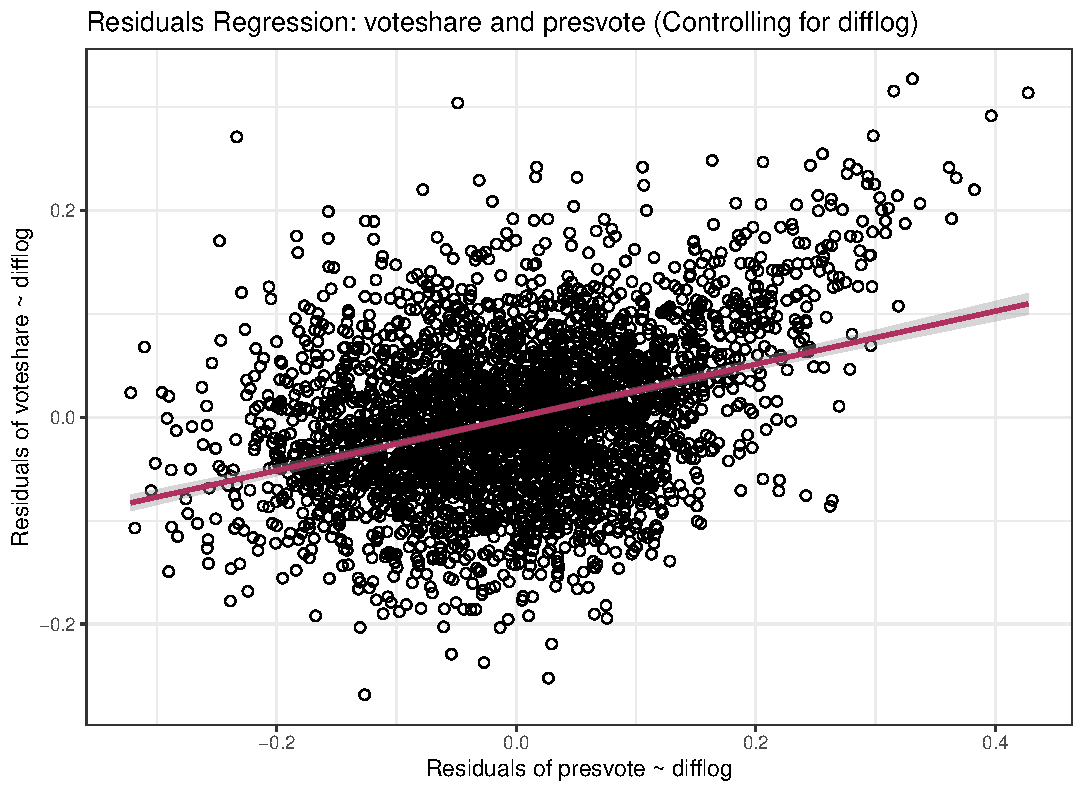
\includegraphics[width=0.8\textwidth]{plot4.pdf} 
		\vspace{.25cm}
		
		
		\item Write the prediction equation.
			\noindent{\texttt{Answer:}} 
		\noindent The prediction equation is: 
		\[
		\widehat{\text{residuals}_1} = 0.000 + 0.257 \times \text{residuals}_2
		\]
	\end{enumerate}
	

\section*{Question 5}
\noindent What if the incumbent's vote share is affected by both the president's popularity and the difference in spending between incumbent and challenger? 
	\begin{enumerate}
		\item Run a regression where the outcome variable is the incumbent's \texttt{voteshare} and the explanatory variables are \texttt{difflog} and \texttt{presvote}.
		
			\noindent{\texttt{Answer:}} 
		\noindent {So, let's run the first regression. }
		\noindent{\texttt{R Code:}} 
		\lstinputlisting[language=R, firstline=172, lastline=173]{PS03_answersSM.R}  
		\noindent {This gives us the following output:}
		
		\begin{table}[!htbp] \centering 
			\caption{} 
			\label{} 
			\begin{tabular}{@{\extracolsep{5pt}}lc} 
				\\[-1.8ex]\hline 
				\hline \\[-1.8ex] 
				& \multicolumn{1}{c}{\textit{Dependent variable:}} \\ 
				\cline{2-2} 
				\\[-1.8ex] & voteshare \\ 
				\hline \\[-1.8ex] 
				difflog & 0.036$^{***}$ \\ 
				& (0.001) \\ 
				& \\ 
				presvote & 0.257$^{***}$ \\ 
				& (0.012) \\ 
				& \\ 
				Constant & 0.449$^{***}$ \\ 
				& (0.006) \\ 
				& \\ 
				\hline \\[-1.8ex] 
				Observations & 3,193 \\ 
				R$^{2}$ & 0.450 \\ 
				Adjusted R$^{2}$ & 0.449 \\ 
				Residual Std. Error & 0.073 (df = 3190) \\ 
				F Statistic & 1,302.947$^{***}$ (df = 2; 3190) \\ 
				\hline 
				\hline \\[-1.8ex] 
				\textit{Note:}  & \multicolumn{1}{r}{$^{*}$p$<$0.1; $^{**}$p$<$0.05; $^{***}$p$<$0.01} \\ 
			\end{tabular} 
		\end{table} 
		
			\noindent {Regressing \textit{voteshare} on both \textit{difflog} and \textit{presvote}, we can see the following: Theoretically, if both explanatory variables equal zero, then the incumbent's vote share is expected to be 44.9\% (which is obviously a very unrealistic scenario).
			Holding the presidential vote share constant, a one-unit increase in the difference in campaign spending between incumbent and challenger is, on average, associated with an increase of 3.6 percentage points in the incumbent’s vote share. In context, holding differences in campaign spending constant, a one-percentage point increase in the presidential candidate’s vote share is, on average, associated with an increase of approximately 0.26 percentage points in the incumbent’s vote share (if i understand how to "convert" the numbers in the dataset to percentages correctly.  I'm not going to lie that took way too long to wrap my head around). Including both explanatory variables, the R-squared value is 0.45. This means that the model explains 45\% of variation in the outcome variable.
			}
		
		\item Write the prediction equation.
		
			\noindent{\texttt{Answer:}} 
		\noindent The prediction equation is: 
		\[
		\widehat{\text{voteshare}} = 0.449 + 0.036 \times \text{difflog} + 0.257 \times \text{presvote}
		\]
		\item What is it in this output that is identical to the output in Question 4? Why do you think this is the case?
		
		\noindent{\texttt{Answer:}} 
		\noindent The slope in Question 4 is equal to the coefficient for \textit{presvote}. That is because both models essentially do the same thing, but use two different approaches. By "taking out"  the variation explained by \textit{difflog} in Question 4, we do the same thing as in the regression for Question 5: controlling for differences in campaign spending. 
		
		We can also compare the scatterplot above with the added variable plot(s) for the model in Question 5:
			\noindent{\texttt{R Code:}} 
		\lstinputlisting[language=R, firstline=177, lastline=179]{PS03_answersSM.R}  
		\noindent {This gives us the following output: {\footnotesize (Admittedly, this would be a better visual guide if the scaling of the graphs was exactly the same, but the point still stands. )}}
		
		
		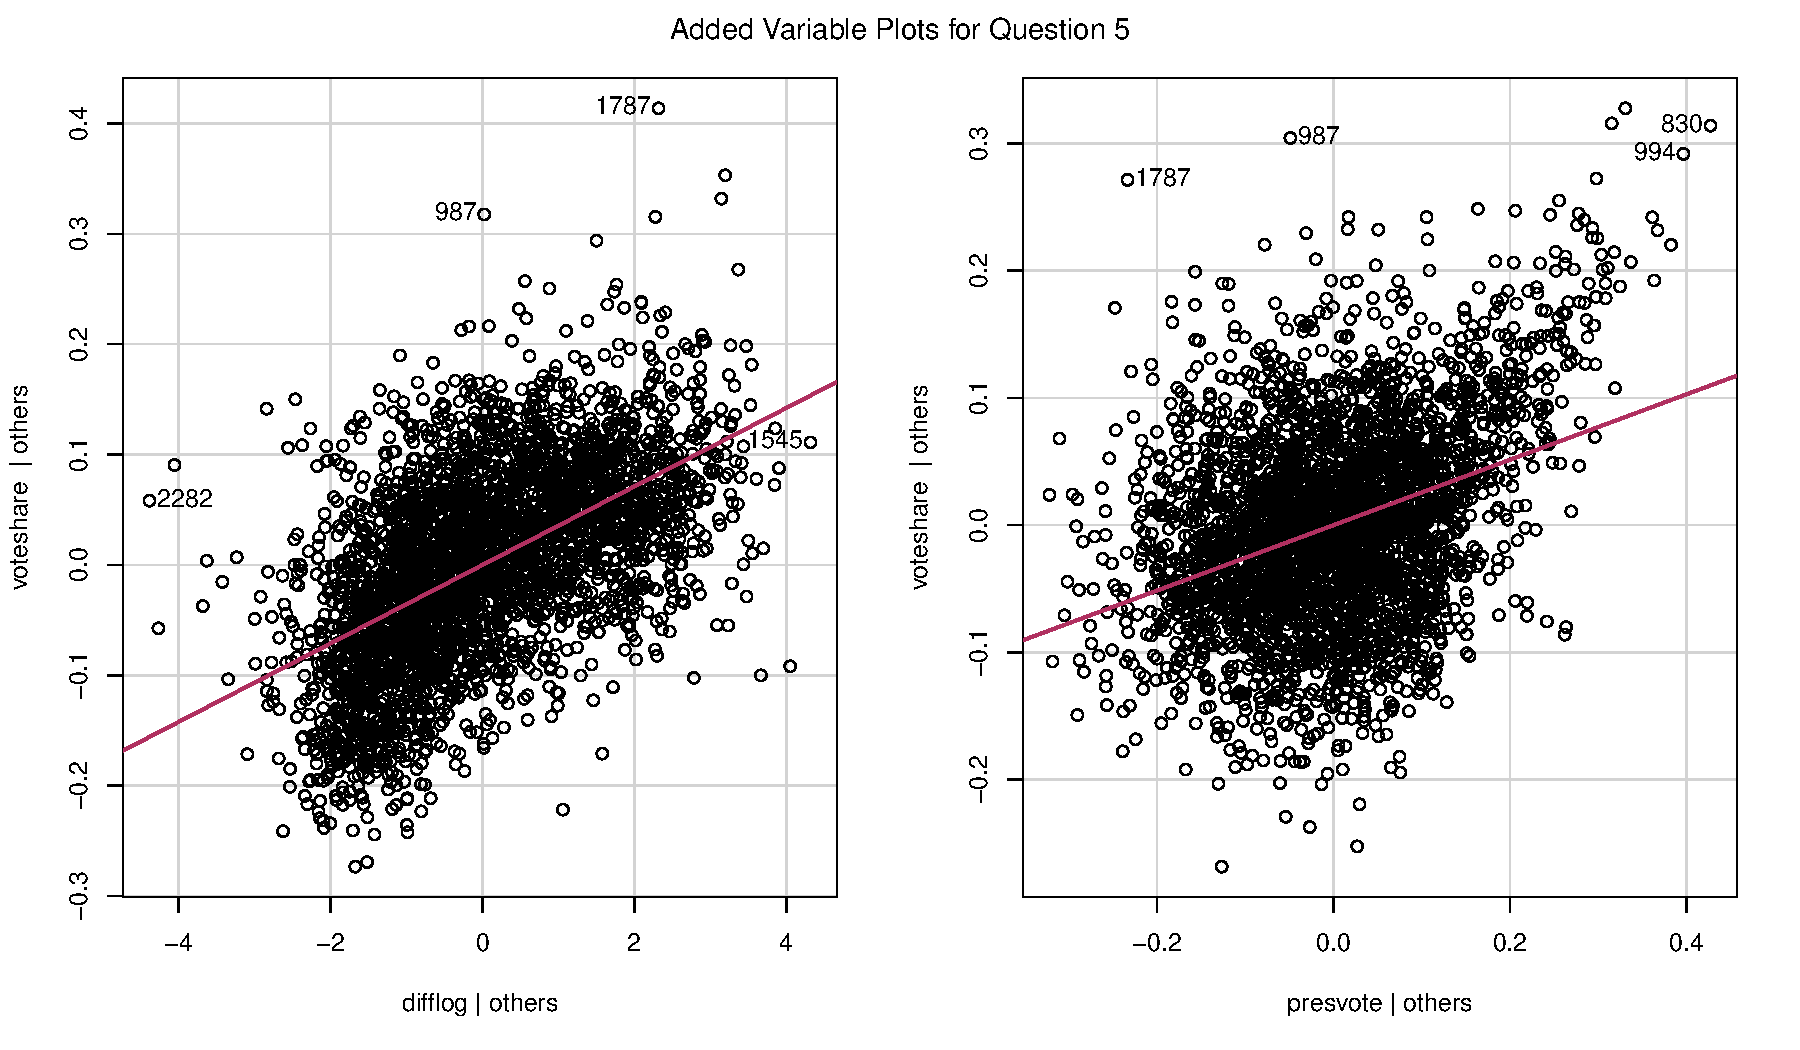
\includegraphics[width=0.8\textwidth]{Added_Variable_Plots_Q5.pdf} 
		
	\end{enumerate}




\end{document}
